\section{Auswertung}
\label{sec:Auswertung}

\begin{figure}
    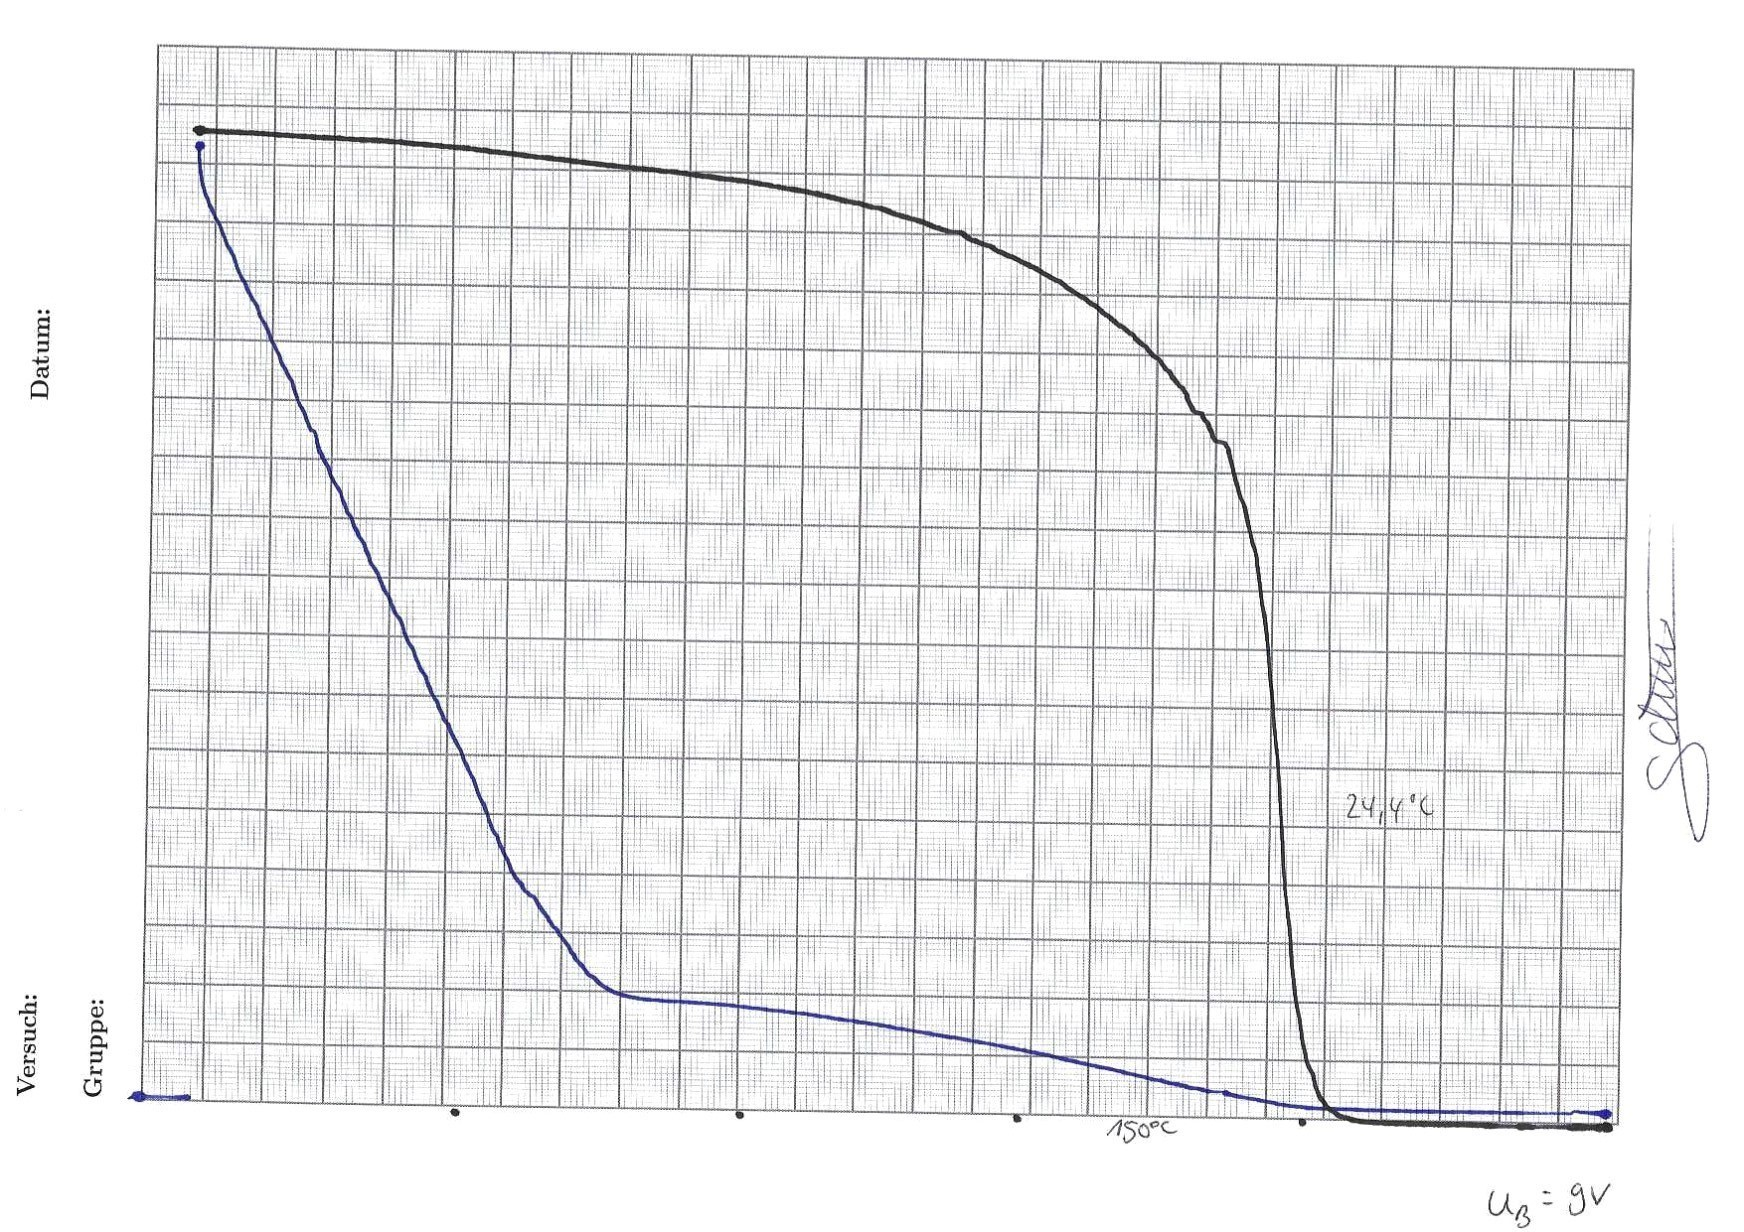
\includegraphics{Bilder/1.jpg}
    \caption{Gemessene Stromstärke gegen die Abbremsspannung bei unterschiedlichen Temparaturen und konstanter Beschleunigungsspannung
    $U_B=\qty{11}{\volt}$.}
    \label{fig:1}
\end{figure}

\begin{figure}
    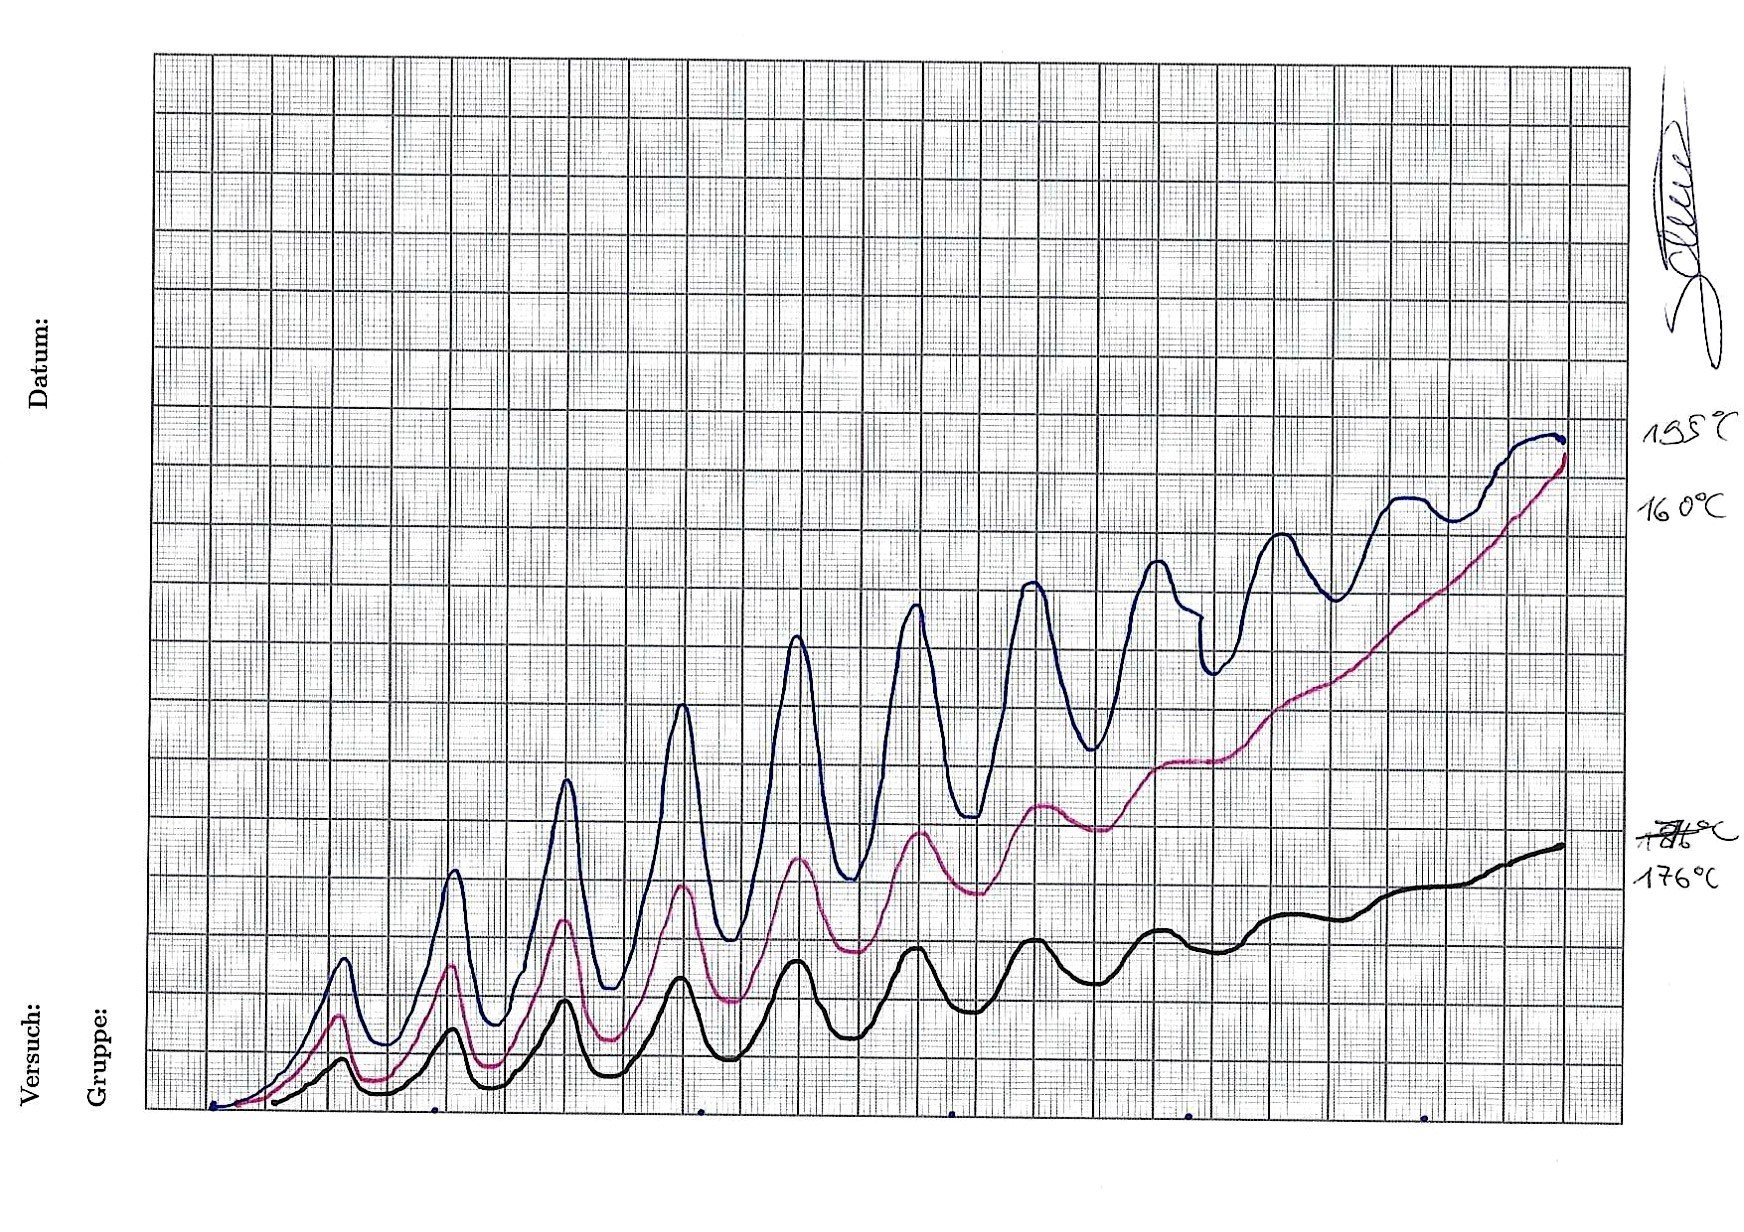
\includegraphics{Bilder/2.jpg}
    \caption{Gemessene Stromstärke gegen die Beschleunigungsspannung bei unterschiedlichen Temparaturen und konstanter Bremsspannung
    $U_A=\qty{1}{\volt}$.}
    \label{fig:2}
\end{figure}

Anhand der Abbildung \ref{fig:2} ist feststellbar, dass der Abstand zwischen den Maxima $d=\qty{2.1}{\centi\meter}$, 
wobei $\qty{1}{\volt}$ etwa $\qty{0.41}{\centi\meter}$ entspricht. Somit beträgt die Spannungsdifferenz $\delta U=\qty{0.861}{\volt}$.

